% ------------------------------------------------------------------------- //
% Facultad de Ingeniería de la Universidad de Buenos Aires
% Algoritmos y Programación II
% 1er Cuatrimestre de 2015
% Trabajo Práctico 1: Recursividad
% Cálculo de DFT
% 
% informe_tp1.tex
% Informe
%
% Para compilar:
% $: pdflatex informe_tp1
% ------------------------------------------------------------------------- //

% ---- Preamble ----
\documentclass{article}


% ---- Packages ----
\usepackage{amsmath} % Advanced math typesetting
\usepackage[utf8]{inputenc} % Unicode support (Umlauts etc.)
\usepackage[spanish]{babel} % Change hyphenation rules
\usepackage{hyperref} % Add a link to your document
\usepackage{graphicx} % Add pictures to your document
\usepackage{float} % For 'H' figure position option. Stricter than 'h!'
%\usepackage{listings} % Source code formatting and highlighting
\usepackage{listingsutf8} % Source code formatting and highlighting in UTF-8
\usepackage[a4paper]{geometry} % Page size options
  \geometry{tmargin=3cm,bmargin=3cm,lmargin=2cm,rmargin=2cm} % Margins
\usepackage{fancyhdr} % Add head­ers and foot­ers
  \setlength{\headheight}{14pt} % Needs to be 13.6pt or more
  \pagestyle{fancy}
  %\fancyhf{} % Clear the default settings
  %\lhead{left header content}
  %\chead{middle header content}
  %\rhead{right header content}
  %\lfoot{left footer content}
  %\cfoot{middle footer content}
  %\rfoot{right footer content}
\usepackage{color} % Colours
  %red, green, blue, yellow, cyan, magenta, black, white
  \definecolor{mygreen}{RGB}{28,172,0} % color values Red, Green, Blue
  \definecolor{mylilas}{RGB}{170,55,241}
  \definecolor{mygray}{rgb}{0.5,0.5,0.5}
  \definecolor{mymauve}{rgb}{0.58,0,0.82}
  \definecolor{myblue}{rgb}{0.33,0.33,0.99}
\hypersetup{ % Remove hyperlink borders
  pdfborder={0 0 0}
}
% ------------------

% ---- Formato para código fuente ----
\lstset{
    language=C++,
    basicstyle=\color{red},
    breaklines=true,%
    morekeywords={matlab2tikz},
    keywordstyle=\color{blue},%
    morekeywords=[2]{1}, keywordstyle=[2]{\color{green}},
    identifierstyle=\color{black},%
    stringstyle=\color{mygreen},
    commentstyle=\color{mygray},%
    showstringspaces=false,%without this there will be a symbol in the places where there is a space
    numbers=left,%
    numberstyle={\tiny \color{mygray}},% size of the numbers
    numbersep=9pt, % this defines how far the numbers are from the text
    emph=[1]{for,end,break},emphstyle=[1]\color{blue}, %some words to emphasise
    emph=[2]{word1,word2}, emphstyle=[2]{style},    
    inputencoding=utf8/latin1, % Para código con tildes y otros caracteres
}
% ------------------------------------


% --------------------------------------------------------------------------- %
% ---- Comienzo del documento ----
\begin{document}

% ---- Carátula ----
\title{Algoritmos y Programación II\\
       TP1: Recursividad}
\author{Bourbon, Rodrigo\\
        Carreño Romano, Carlos Germán\\
        Sampayo, Sebastián Lucas}
\date{Primer Cuatrimestre de 2015}
\maketitle

\begin{center}
  
\includegraphics[width=0.5\paperwidth]{Imagenes/logo_fiuba_HD}
  %\rule[depth]{width}{height}
  \rule[0.5ex]{0.8\paperwidth}{0.1pt}
\par
\end{center}

\pagenumbering{gobble} % Don't number this page
% ------------------

% ---- Encabezado ----
\lhead{Algoritmos y Programación II - TP1 - FIUBA}
% --------------------

% ---- Tabla de contenidos ----
\newpage{}
\vfill{}
\tableofcontents{}
\vfill{}
\newpage{}
% -----------------------------
% ------------------------------------
\pagenumbering{arabic} % Do number this page, arabic numbers


\section{Objetivos}
  Ejercitar técnicas de diseño, análisis, e implementación de algoritmos recursivos.

\section{Introducción}
  Explicar un poco que es la FT, la DFT y la FFT.

\section{Standard de estilo}
  Adoptamos la convención de estilo de código de Google para C++, salvando las siguientes excepciones:
  \begin{itemize}
    \item Streams: utilizamos flujos de entrada y salida
    \item Sobrecarga de operadores
  \end{itemize}
  \url{https://google-styleguide.googlecode.com/svn/trunk/cppguide.html#Naming}

\section{Diseño del programa}
  Explicar a grandes rasgos como funciona el programa, diagrama en bloques.
  -> Leer de la entrada a vector, rellenar con ceros, transformar, imprimir vector.

\section{Opciones del programa}
  El programa se ejecuta en línea de comandos, y las opciones que admite (sin importar el orden de aparición) son las siguientes:
  \begin{itemize}
    \item[] \textit{nombre largo} (\textit{nombre corto}): \textit{descripción}
    \item \texttt{--input} (\texttt{-i}): 
    
    En esta opción se indica un argumento que debe ser la ruta de un archivo del cual queramos leer o bien la opción por defecto ”-” que utiliza el flujo de entrada estándar.
    \item \texttt{--output} (\texttt{-o}): 
    
    En esta opción se indica un argumento que debe ser la ruta de un archivo en el cual queramos imprimir o bien la opción por defecto ”-” que utiliza el flujo de salida estándar.
    \item \texttt{--method} (\texttt{-m}): 
    
    En esta opción se indica la acción que se debe realizar sobre los datos de la entrada, estos pueden ser:
    \begin{itemize}
    \item[•]Transformada discreta de Fourier (\texttt{-dft}).
    \item[•]Transformada discreta inversa de Fourier (\texttt{-idft}).
    \item[•]Transformada rápida de Fourier (\texttt{-fft}).
    \item[•]Transformada rápida inversa de Fourier (\texttt{-ifft}).
    
    \end{itemize}
    Por defecto el programa se ejecuta con la transformada rápida de fourier.
  \end{itemize}

\section{Métodos de la Transformada}
  como fue implementado dft y fft, funciones genéricas, máscaras, complejidad temporal, espacial, etc.
  \subsection{FFT}
    \subsubsection{Complejidad Temporal}
      Para estudiar el costo temporal de esta implementación ---$T(N)$--- se analizó
    cada línea de código de la función \textit{calculate\_fft\_generic()}.\par
    Al principio, todas las sentencias son de orden constante hasta que
    aparece el primer ciclo:
      %copiar una vez tengamos la versión final
    \lstinputlisting{calculate_fft_1.cc}
%    \begin{lstlisting}
%    \end{lstlisting}
      Las únicas expresiones que ofrecen cierta duda de que su coste sea 
    constante son las últimas ---constructores de N/2 elementos. Sin embargo,
    al ver la implementación de dicho constructor no quedan dudas, ya que solo
    consiste en una comparación, una asignación, y una llamada a \textit{new}:
      % copiar código función Vector(int)
    \lstinputlisting{Vector_int_ctor.cc}
%    \begin{lstlisting}
%    \end{lstlisting}
      Continuando con la función \textit{calculate\_fft\_generic()} :
    \lstinputlisting{calculate_fft_2.cc}
      Se tiene un ciclo de N/2 iteraciones cuyas operaciones en cada caso
    son de orden constante, con lo cual el orden de este ciclo es $\mathcal{O}(N/2)$. \par
      %copiar una vez tengamos la versión final
%    \begin{lstlisting}
%    \end{lstlisting}
      A continuación encontramos las llamadas recursivas. Dado que el tamaño
     de la entrada se reduce a la mitad, tenemos 2 llamadas de coste $T(N/2)$. \par
      %copiar una vez tengamos la versión final
%    \begin{lstlisting}
%    \end{lstlisting}
      Finalmente, se tiene un ciclo de N iteraciones cuyas operaciones en cada 
    caso son de orden constante, produciendo un coste de $\mathcal{O}(N)$.
      %copiar una vez tengamos la versión final
%    \begin{lstlisting}
%    \end{lstlisting}
      De esta forma, agrupando estos resultados parciales, se puede escribir la
     ecuación de recurrencia para este algoritmo:
    \begin{align*}
      T(N) &= \mathcal{O}(1) + \mathcal{O}(N/2) + 2T(N/2) + \mathcal{O}(N) \\
      T(N) &= 1 + N + 2T(N/2) \\
    \end{align*}
    \begin{equation*}
      \boxed{T(N) = 2T(N/2) + N}
    \end{equation*}
      Como se puede ver, es posible aplicar el teorema maestro, definiendo:
    \begin{align*}
      a &= 2 \geq 1 \\
      b &= 2 > 1\\
   f(N) &= N
    \end{align*}
      Utilizando el segundo caso del teorema:
    $$ \exists\,k \geq 0 \quad / \quad N \;\epsilon\; \Theta (N^{\log_b (a)} \log^k (N)) $$
    $$ \Rightarrow T(N)\;\epsilon\;\Theta (N^{\log_b (a)} \log^{k+1} (N)) $$
      Es fácil ver que con $k=0$ dicha condición se cumple, por lo tanto
    el resultado final es:
    $$ \boxed{T(N)\;\epsilon\;\Theta (N \log N)} $$
      Este resultado es coherente, ya que el algoritmo utiliza la técnica de 
    "divide y vencerás" y la recurrencia es análoga al caso del conocido 
    \textit{MergeSort}.
    
    \subsection{DFT}
    \subsubsection{Complejidad Temporal}
      Para estudiar el costo temporal de esta implementación ---$T(N)$--- se analizó
    cada línea de código de la función \textit{calculate\_dft\_generic()}.\par
    Al principio, todas las sentencias son de orden constante hasta que
    aparece el primer ciclo de N iteraciones. Dentro de este hay otro cilco de N 
  iteraciones y 2 sentencias de orden constante, mientras que en el ciclo anidado 
  hay una llamada a una funcion recursiva (\textit{pow\_Complex}):
  \lstinputlisting{calculate_dft.cc}
  Analizamos el coste temporal ---$T_p(p)$--- de la función (\textit{pow\_Complex}):
  \lstinputlisting{pow_complex.cc}
    Se observa que todas las operaciones son de orden constante $\mathcal{O}(1)$ 
    y a continuación se tiene una llamada recursiva. Dado que el tamaño del problema se reduce 
    a la mitad, tenemos 1 llamada de coste $T_p(p/2)$
    Agrupando estos resultados, se puede escribir la
      ecuación de recurrencia para este algoritmo:
    \begin{align*}
      T_p(p) &= \mathcal{O}(1) + T_p(p/2)\\
  \end{align*}
      \begin{equation*}
        \boxed{T_p(p) = T_p(p/2) + 1}
      \end{equation*}
    
    Como se puede ver, es posible aplicar el teorema maestro, definiendo:
    \begin{align*}
      a &= 1 \geq 1 \\
      b &= 2 > 1\\
   f(p) &= 1 
    \end{align*}
      Utilizando el segundo caso del teorema:
    $$ \exists\,k \geq 0 \quad / \quad f(p) \;\epsilon\; \Theta (p^{\log_b (a)} \log^k (p)) $$
    $$ \Rightarrow T_p(p)\;\epsilon\;\Theta (p^{\log_b (a)} \log^{k+1} (p)) $$
      Es fácil ver que con $k=0$ dicha condición se cumple, por lo tanto
    el resultado final es:
    $$ T_p(p)\;\epsilon\;\Theta (\log p) $$\\
  Una vez sabido el coste temporal de este algoritmo podemos calcular el de la función
  principal. Como se había planteado anteriormente, consta de 2 ciclos anidados de N iteraciones.
  El coste del segundo ciclo está dado por:
  \begin{align*}
      T(N) &= (\mathcal{O}(1) + {\Theta}(\log N)) * N
  \end{align*}
    $$ \Rightarrow T(N)\;\epsilon\;\Theta (N\log N) $$
  Entonces el coste total del primer ciclo es:
  \begin{align*}
      T(N) &= (\mathcal{O}(1) + {\Theta}(N\log N)) * N
  \end{align*}
  $$ \Rightarrow T(N)\;\epsilon\;\Theta (N^2\log N) $$
  Juntando todos los resultados parciales tenemos que el coste total del algoritmo es:
  \begin{align*}
      T(N) &= \mathcal{O}(1) + {\Theta}(N^2\log N)
  \end{align*}
  $$ \Rightarrow \boxed{ T(N)\;\epsilon\;\Theta (N^2\log N) } $$
    En conclusión se puede ver que si la función \textit{pow\_Complex()} fuera reemplazada por
  una expresión de orden constante (como por ejemplo la creación del número complejo W
  directamente en cada iteración, como se hizo en la implementación de la FFT), entonces se 
  perdería la componente logarítmica de la complejidad, quedando el resultado final:
  $$ \boxed{ T(N)\;\epsilon\;\Theta (N^2) } $$



\section{Estructura de archivos}

\begin{center}
  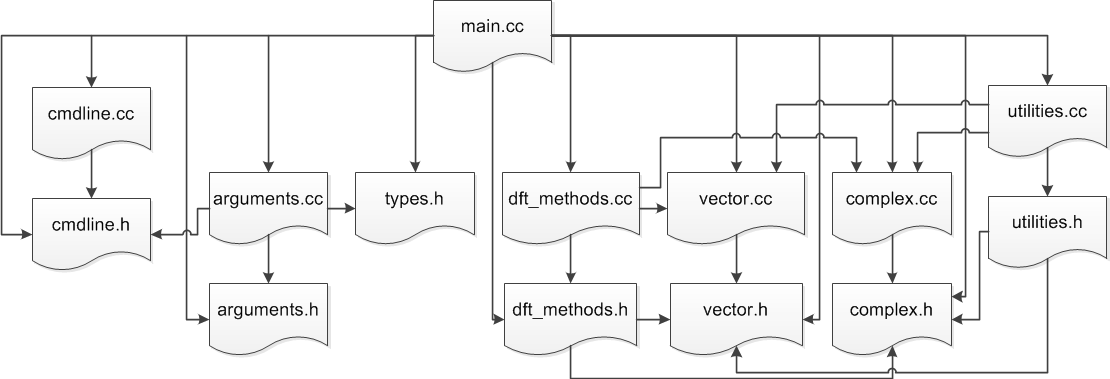
\includegraphics[width=0.8\paperwidth]{Imagenes/jerarquia_de_archivos}
\par
\end{center}

\section{Compilación}
Como se compila

\section{Casos de prueba}

Se realizó un \textit{script} para la ejecución de todos los casos de prueba.
\lstinputlisting{test_especificacion.sh} \par
  \subsection{Caso 1}
    \begin{center}
      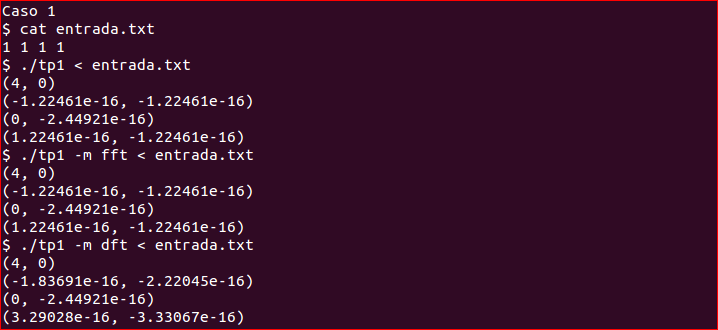
\includegraphics[width=0.8\paperwidth]{Imagenes/caso_1}
    \end{center}
  \subsection{Caso 2}
    \begin{center}
      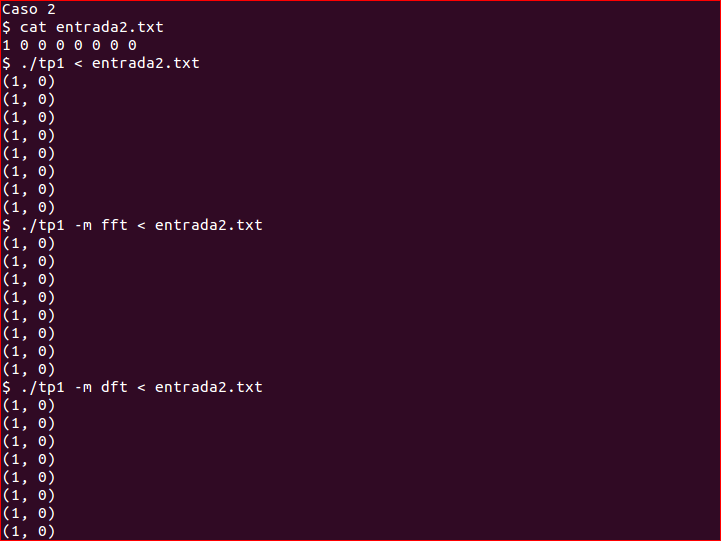
\includegraphics[width=0.8\paperwidth]{Imagenes/caso_2}
    \end{center}
  \subsection{Caso 3}
    
  \subsection{Caso 4}
    \begin{center}
      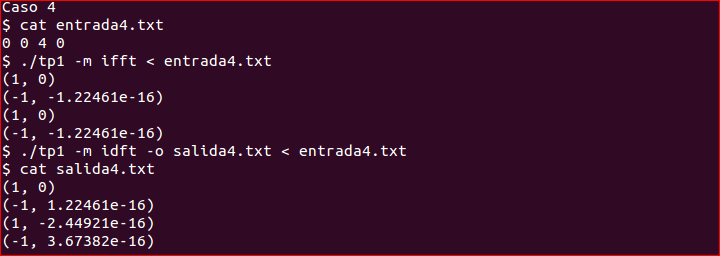
\includegraphics[width=0.8\paperwidth]{Imagenes/caso_4}
    \end{center}

\section{Código}

% Plantilla de figura:
%  \begin{figure}[H]
%  \begin{centering}
%  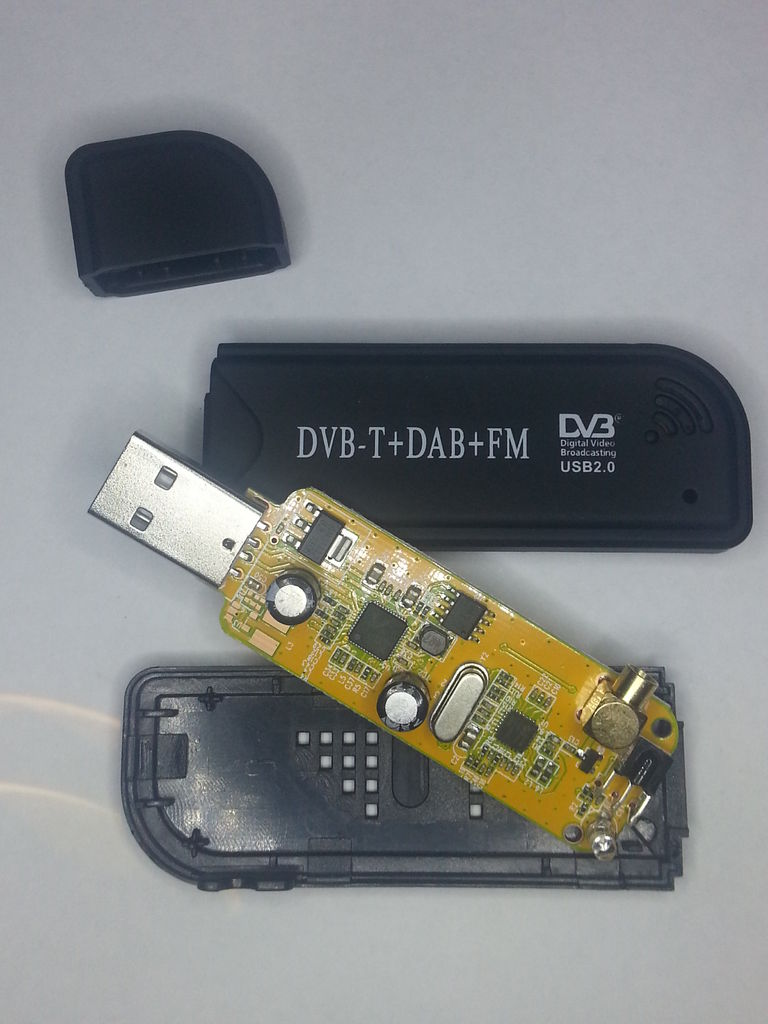
\includegraphics[width=0.75\textwidth]{Imagenes/SDR.jpg}
%  \par\end{centering}
%  \caption{Sintonizador de radio digital.}
%  \end{figure}

% Plantilla de código fuente:
%    \lstinputlisting{code.cc}

\section{Enunciado}

\end{document}
